\documentclass[10pt,conference]{IEEEtran}
\IEEEoverridecommandlockouts

% --- packages ---
\usepackage{graphicx}
\usepackage{tikz}
\usetikzlibrary{positioning,fit,arrows.meta,calc}
\usepackage{pgfplots}
\pgfplotsset{compat=1.18} % 標準設定(目盛り方向などは変更しない)
\usepackage{amsmath}
\usepackage{booktabs}
\usepackage{cite}
\usepackage{balance}
\usepackage[hidelinks]{hyperref} % ← できるだけ最後に

% --- title/author ---
\title{LPDDR+FeRAM for Mobile Edge AI:\\
Chiplet/SiP Integration as a Practical Path}

\author{%
  \IEEEauthorblockN{Shinichi Samizo}%
  \IEEEauthorblockA{Independent Semiconductor Researcher\\
  Former Engineer, Seiko Epson Corporation\\
  Email: \href{mailto:shin3t72@gmail.com}{shin3t72@gmail.com}\\
  GitHub: \href{https://github.com/Samizo-AITL}{Samizo-AITL}}%
}

\begin{document}
\maketitle

% ===== Abstract =====
\begin{abstract}
Low-power DRAM (LPDDR) is the dominant main memory for mobile edge AI accelerators, balancing bandwidth and energy efficiency. 
However, LPDDR remains volatile and incurs standby power due to periodic refresh. 
Ferroelectric RAM (FeRAM), based on HfO$_2$, provides non-volatility, low-voltage operation, and fast rewriting, making it suitable as an assistive memory for checkpointing and state retention. 
Because monolithic LPDDR+FeRAM co-fabrication is infeasible due to process--temperature mismatch, this work proposes \textbf{chiplet-level LPDDR+FeRAM integration} using SiP/PoP packaging. 

System-level analysis, based on representative LPDDR5/5X and HfO$_2$-FeRAM parameters from prior silicon reports, shows that FeRAM chiplets can reduce standby power by up to 20\%, shorten resume latency from $\sim$10~ms (baseline LPDDR) to sub-ms range ($<$500~$\mu$s), and improve overall energy efficiency by 15--25\% under mobile edge AI workloads such as on-device inference, federated learning, and AR/VR. 
These results are derived from analytical modeling rather than prototype measurements, positioning the study as a \emph{design framework exploration} rather than a device demonstration.

The proposed architecture is coordinated by the \textbf{SystemDK co-design framework}, which manages checkpoint and refresh-offload policies across architecture, package, and runtime layers. 
\textbf{Target implementation nodes:} SoC at 5--3\,nm (FinFET/GAAFET), LPDDR5/5X at 1$\alpha$--1$\gamma$ DRAM nodes ($\sim$14--10\,nm), and a 28--22\,nm CMOS FeRAM chiplet integrated via SiP/PoP. 
This approach highlights a near-term, manufacturable path toward energy-efficient and responsive memory subsystems, while providing an educational reference for heterogeneous memory integration.
\end{abstract}

% ===== Sections =====
\begin{abstract}
High-bandwidth memory (HBM) provides the throughput required by mobile edge AI accelerators but suffers from high standby power due to periodic refresh and volatility. 
Ferroelectric memories (FeRAM/FeFET), based on HfO$_2$, provide non-volatility and fast write, though at higher energy cost. 
This work explores hybrid integration of HBM and FeRAM/FeFET: near-term chiplet-based co-packaging and long-term monolithic prospects. 
Results show that FeRAM integration enables standby reduction and instant resume, while FeFET offers future scalability for dense, non-volatile HBM.
\end{abstract}

\section{Introduction}
Mobile edge AI requires memory systems that combine:
(1) multi-hundred GB/s bandwidth, 
(2) low standby power, 
(3) instant resume after power gating, 
and (4) endurance for frequent checkpoints.
HBM DRAM meets (1) but fails in (2--3), as refresh consumes significant standby power. 
Ferroelectric RAM (FeRAM) and FeFET devices, based on ferroelectric HfO$_2$, inherently provide (2--3), with endurance of $10^{12}$–$10^{13}$ cycles \cite{MuellerIEDM2012,MartinVLSI2020}. 
This paper evaluates hybrid HBM+FeRAM/FeFET integration, considering both chiplet co-packaging and monolithic process feasibility.
 

\section{Device and Process Integration}
HBM DRAM stacks are typically fabricated with high-temperature capacitor anneals ($>700~^\circ$C), 
whereas FeRAM/FeFET devices require lower-temperature processing ($\sim$400~^\circ$C) to stabilize the ferroelectric o-phase in HfO$_2$. 
This incompatibility between high- and low-temperature requirements currently hinders monolithic integration.

\subsection{Chiplet-based Integration (Practical Solution)}
The most practical near-term approach is chiplet-based integration:  
HBM stacks and FeRAM/FeFET dies are fabricated in their respective optimized flows and co-integrated on a silicon interposer using $\mu$-bump connections.  
This architecture enables:
\begin{itemize}
  \item High-bandwidth operation from HBM ($>$300~GB/s),
  \item Persistent storage of checkpoints, metadata, and cold data in FeRAM,
  \item Reduction of refresh-induced traffic in DRAM.
\end{itemize}

\subsection{Monolithic Integration (Research Challenge)}
A longer-term research direction is embedding FeFET arrays within the HBM logic base die.  
In principle, DRAM capacitor HfO$_2$ and FeFET gate-stack HfO$_2$ could coexist; however, their annealing requirements remain incompatible.  
Possible enablers include selective or dual-step annealing, dopant modulation, or stress engineering.  
At present, monolithic HBM+FeFET integration remains an open challenge for device and process research.

% ===== Fig.1: System-level schematic with SystemDK (TikZ) =====
\begin{figure}[!t]
\centering
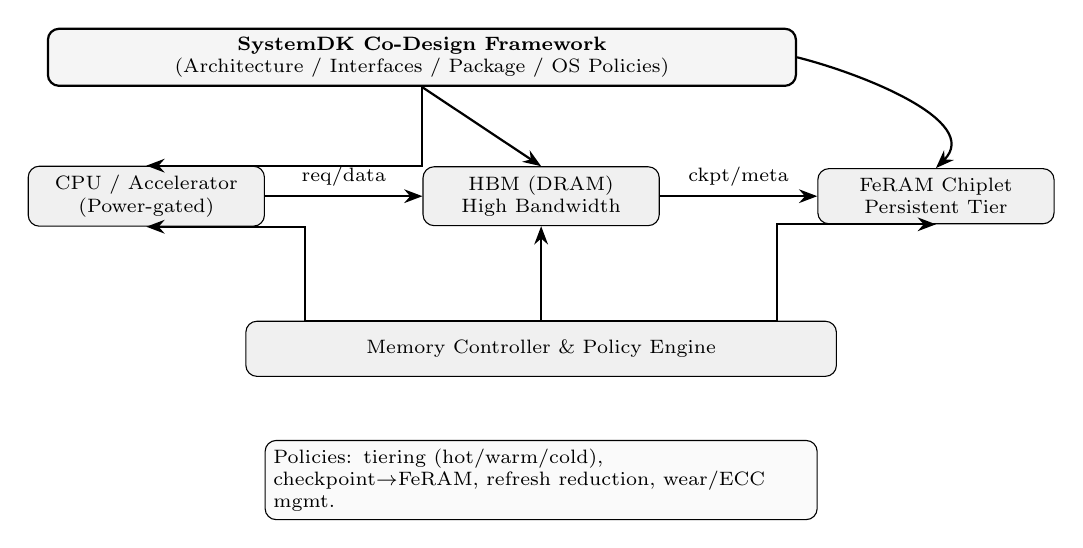
\begin{tikzpicture}[font=\scriptsize, >=Stealth, node distance=1.0cm]
  % Styles
  \tikzset{
    blk/.style={draw=black, rounded corners, fill=black!6, minimum width=3.0cm, minimum height=7mm, align=center},
    note/.style={draw=black, rounded corners, fill=black!2, align=left, inner sep=3pt, text width=6.8cm},
    arrow/.style={->, thick},
    sysdk/.style={draw=black, thick, rounded corners, fill=black!4, align=center, inner sep=3pt, minimum width=9.5cm}
  }

  % SystemDK box
  \node[sysdk] (sdk) {\textbf{SystemDK Co-Design Framework}\\
  (Architecture / Interfaces / Package / OS Policies)};

  % Main blocks
  \node[blk, below=1.0cm of sdk, xshift=-3.5cm] (cpu) {CPU / Accelerator\\(Power-gated)};
  \node[blk, right=2.0cm of cpu] (hbm) {HBM (DRAM)\\High Bandwidth};
  \node[blk, right=2.0cm of hbm] (feram) {FeRAM Chiplet\\Persistent Tier};

  % Controller
  \node[blk, below=1.2cm of hbm, minimum width=7.5cm] (ctrl) {Memory Controller \& Policy Engine};

  % Policies note(簡略化)
  \node[note, below=0.8cm of ctrl] (pol) {
    Policies: tiering (hot/warm/cold), checkpoint$\to$FeRAM, refresh reduction, wear/ECC mgmt.
  };

  % Data arrows
  \draw[arrow] (cpu) -- node[above]{req/data} (hbm);
  \draw[arrow] (hbm) -- node[above]{ckpt/meta} (feram);
  \draw[arrow] (ctrl.north) -- ++(-3.0,0) |- (cpu.south);
  \draw[arrow] (ctrl.north) -- (hbm.south);
  \draw[arrow] (ctrl.north) -- ++(3.0,0) |- (feram.south);

  % SystemDK supervision arrows
  \draw[arrow] (sdk.south) |- (cpu.north);
  \draw[arrow] (sdk.south) -- (hbm.north);
  \draw[arrow] (sdk.east) .. controls +(0.8,-0.2) and +(0.6,0.6) .. (feram.north);
\end{tikzpicture}
\caption{Chiplet-level integration supervised by \textbf{SystemDK}. CPU/Accelerator, HBM, and FeRAM chiplet co-integrated on an interposer.}
\label{fig:system_schematic_sdk}
\end{figure}

\section{Failure Analysis and Yield Improvement}

\subsection{Initial Observation}
The first production lots showed $\sim$65\% yield. Wafer test was dominated by \textbf{Pause Refresh Fail (Bin5)}. Defects appeared as uniformly scattered single-bit errors across the wafer (weak clustering, no edge/line signature). Storage-node capacitance met spec; SEM cross-sections at failed cells revealed no structural anomaly. Other CDs/films/electricals were within spec.

\begin{figure}[t]
  \centering
  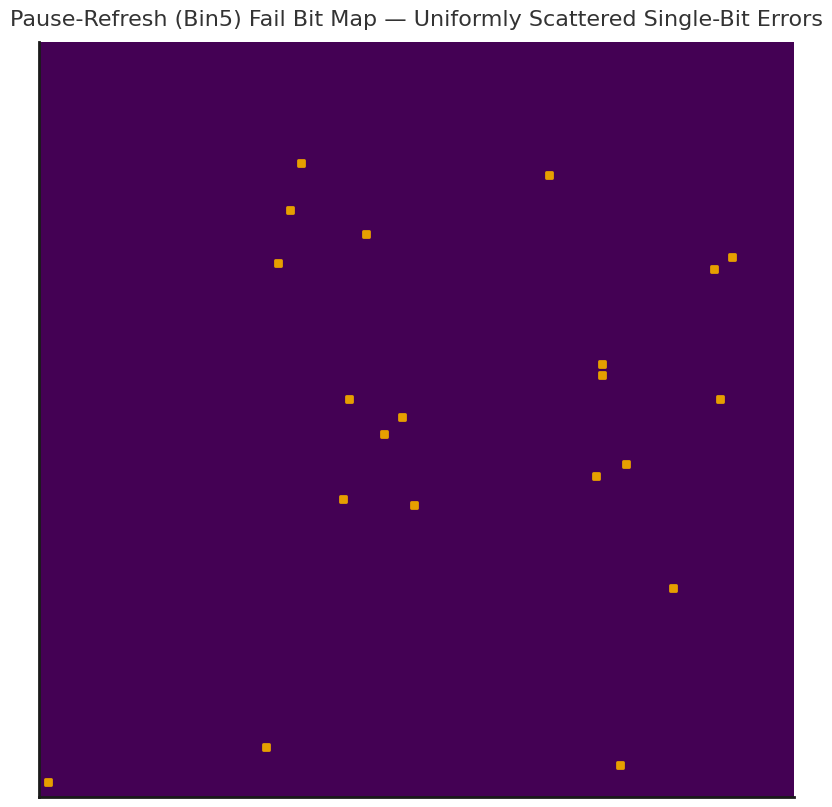
\includegraphics[width=\columnwidth]{fail_bitmap_bin5}
  \caption{Typical fail bit map under pause-refresh test (Bin5).
  Uniformly scattered single-bit errors are observed without edge/line signatures.}
  \label{fig:fail_bitmap}
\end{figure}

\subsection{Hypothesis (Failure Model)}
Directly measurable leakages were normal, suggesting a subtle leakage path. We hypothesized increased leakage at the \textbf{storage-node contact $n^+/p^-$ junction}. After gate etch, a remnant gate oxide on S/D active is repeatedly exposed to resist-stripping \emph{ashing} during multiple LDD steps. Cumulative plasma damage makes the oxide locally porous and can extend damage into the diffusion, creating minute leakage paths. This explains random single-bit distribution without visible structural defects.

% === Storage-node contact n+/p- leakage (TikZ) ===
% === Fig.2 Storage-node contact n+/p- leakage (pure TikZ, minimal IEEE style) ===
\begin{figure}[t]
\centering
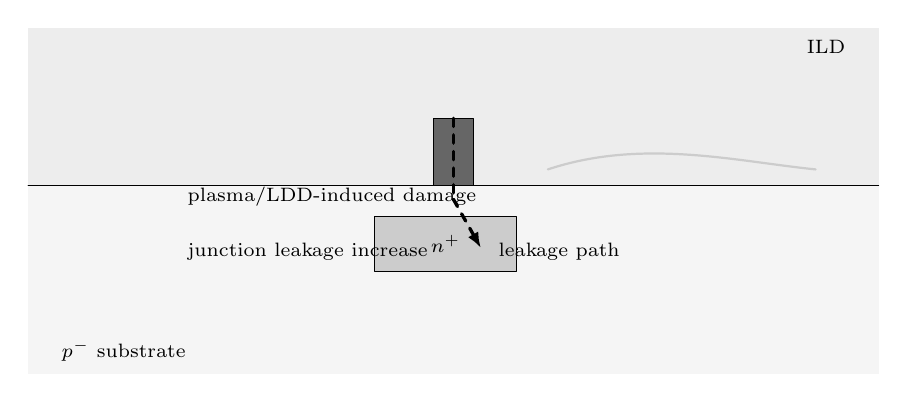
\begin{tikzpicture}[x=1cm,y=1cm,line cap=round,line join=round]
  % 色(グレースケール)
  \def\colILD{black!7}    % ILD淡グレー
  \def\colSub{black!4}    % p-基板の淡グレー
  \def\colDiff{black!20}  % n+拡散
  \def\colLOCOS{black!20} % LOCOS輪郭
  \def\colMetal{black!60} % 金属プラグ

  % キャンバス範囲
  \path (-4.8,-2.4) rectangle (6.0,2.0);

  % ---- ILD(上部帯)----
  \fill[\colILD] (-4.8,0) rectangle (6.0,2.0);
  \node[anchor=east, font=\scriptsize] at (5.7,1.75) {ILD};

  % ---- 基板と表面 ----
  \fill[\colSub] (-4.8,-2.4) rectangle (6.0,0);
  \draw (-4.8,0) -- (6.0,0);
  \node[anchor=west, font=\scriptsize] at (-4.5,-2.1) {$p^{-}$ substrate};

  % ---- LOCOS(右側の鳥のくちばし風プロファイル)----
  \draw[\colLOCOS, line width=0.8pt]
    (1.8,0.20) .. controls (3.0,0.60) and (4.2,0.30) .. (5.2,0.20);

  % ---- n+拡散(ストレージ側)----
  \fill[\colDiff] ( -0.4,-1.1) rectangle (1.4,-0.4);
  \draw ( -0.4,-1.1) rectangle (1.4,-0.4);
  \node[font=\scriptsize] at (0.5,-0.75) {$n^{+}$};

  % ---- ストレージノード・コンタクトプラグ ----
  \fill[\colMetal] (0.35,0.00) rectangle (0.85,0.85);
  \draw (0.35,0.00) rectangle (0.85,0.85);

  % ---- 破線リークパス(コンタクト端→接合)----
  \draw[very thick, dashed] (0.60,0.85) -- (0.60,-0.18);
  \draw[very thick, dashed, -{Latex[length=2mm]}] (0.60,-0.18) -- (0.95,-0.80);
  \node[anchor=west, font=\scriptsize] at (1.05,-0.85) {leakage path};

  % ---- 注記(最小限)----
  \node[anchor=west, font=\scriptsize] at (-2.9,-0.15) {plasma/LDD-induced damage};
  \node[anchor=west, font=\scriptsize] at (-2.9,-0.85) {junction leakage increase};
\end{tikzpicture}
\caption{Schematic of storage-node contact (n$^+$/p$^-$) leakage.
Damage near the contact edge increases junction leakage, degrading retention.}
\label{fig:storage_contact}
\end{figure}

\subsection{Countermeasures}
\begin{itemize}
  \item \textbf{Process}: Replace resist stripping in LDD steps from plasma ashing to \textbf{wet stripping (sulfuric-based)} to eliminate plasma damage. 
  \item \textbf{Integration hygiene}: Confirm downstream photo cleanliness and avoid residue risks with the wet strip.
\end{itemize}

\subsection{Effectiveness}
Yield improved from $\sim$65\% to \textbf{$\sim$80\%}. Uniformly scattered single-bit fails decreased markedly. Burn-in and retention/reliability passed; the final recipe was fixed for volume production.

% === Yield-by-lot (step improvement at countermeasure) ===
\begin{figure}[t]
\centering
\pgfplotstableread[col sep=comma]{data/yield_lot.csv}\yieldtbl
\begin{tikzpicture}
\begin{axis}[
  width=\columnwidth, height=0.58\columnwidth,
  xlabel={Lot ID}, ylabel={Yield [\%]},
  ymin=50, ymax=95,
  xmin=0.5, xmax=12.5,
  grid=both,
  xtick=data,
  xticklabels from table={\yieldtbl}{lot},
  xticklabel style={rotate=45, anchor=east},
]
  % データ描画
  \addplot+[mark=*] table[x expr=\coordindex+1, y=yield]{\yieldtbl};

  % 対策境界: lot04とlot05の間
  \draw[dashed] (axis cs:4.5,50) -- (axis cs:4.5,95);
  \node[anchor=west, font=\footnotesize] at (axis cs:4.55,92)
    {Countermeasure};
\end{axis}
\end{tikzpicture}
\caption{Yield step improvement at the countermeasure boundary
between \texttt{lot04} and \texttt{lot05}. Yield jumps from $\sim$62--63\% 
(lot01--lot04) to $\sim$82--84\% (lot05 onward) after changing 
LDD resist stripping from ashing to wet stripping.}
\label{fig:yield}
\end{figure}

\section{Future Outlook: Toward HBM+FeFET}
In the near term, chiplet integration of HBM and FeRAM offers a practical solution for mobile edge AI, balancing bandwidth and persistence. 
Future prospects include replacing FeRAM with FeFET:
\begin{itemize}
  \item \textbf{Non-destructive read}, reducing wear-out,
  \item \textbf{Higher density}, fitting within HBM logic base,
  \item \textbf{CMOS compatibility}, easing scaling to advanced nodes.
\end{itemize}

Nevertheless, true monolithic integration faces process conflicts: DRAM capacitors require high-$T$ anneals, while FeFETs demand low-$T$ stabilization. 
Overcoming this is an active research challenge.

% ===== Fig.3: Package cross-section with SystemDK (TikZ) =====
\begin{figure}[!t]
\centering
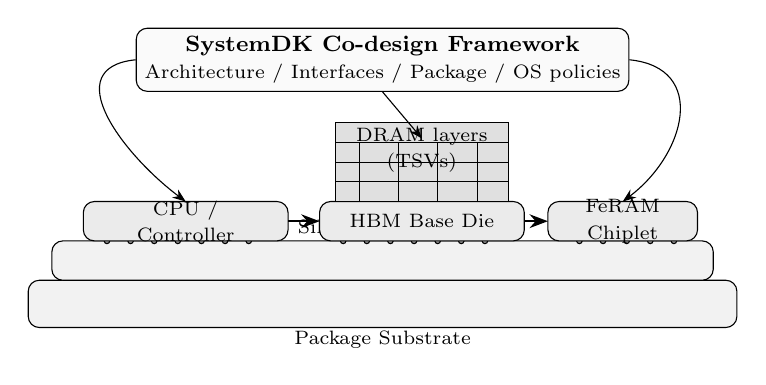
\begin{tikzpicture}[font=\footnotesize, x=1cm, y=1cm, >=Stealth]
  \tikzset{
    layer/.style={draw=black, fill=black!5, rounded corners},
    die/.style={draw=black, fill=black!8, rounded corners},
    stack/.style={draw=black, fill=black!12},
    bump/.style={circle, draw=black, fill=black!40, minimum size=2pt, inner sep=0pt},
    tsv/.style={draw=black, line width=0.3pt},
    sysdk/.style={draw=black, rounded corners, fill=black!2, align=center, inner sep=3pt}
  }
  % SystemDK label
  \node[sysdk] (sdk) at (0,1.2) {\textbf{SystemDK Co-design Framework}\\
    \scriptsize Architecture / Interfaces / Package / OS policies};
  % substrate & interposer
  \draw[layer] (-4.5,-2.2) rectangle (4.5,-1.6);
  \node at (0,-2.35) {\scriptsize Package Substrate};
  \draw[layer] (-4.2,-1.6) rectangle (4.2,-1.1);
  \node at (0,-0.95) {\scriptsize Silicon Interposer};
  % micro-bumps
  \foreach \x in {-3.5,-3.2,...,-1.5} \node[bump] at (\x,-1.1) {};
  \foreach \x in {-0.5,-0.2,...,1.5}  \node[bump] at (\x,-1.1) {};
  \foreach \x in {2.5,2.8,...,3.9}     \node[bump] at (\x,-1.1) {};
  % dies
  \draw[die] (-3.8,-0.6) rectangle (-1.2,-1.1);
  \node[align=center] at (-2.5,-0.85) {\scriptsize CPU /\\ \scriptsize Controller};
  \draw[die] (-0.8,-0.6) rectangle (1.8,-1.1);
  \node at (0.5,-0.85) {\scriptsize HBM Base Die};
  % HBM stacks + TSVs
  \foreach \y in {0.0,0.25,0.50,0.75} {
    \draw[stack] (-0.6,\y-0.6) rectangle (1.6,\y-0.35);
  }
  \foreach \x in {-0.3, 0.2, 0.7, 1.2}{
    \draw[tsv] (\x,-0.6) -- (\x,0.15);
  }
  \node[align=center] at (0.5,0.05) {\scriptsize DRAM layers\\ \scriptsize (TSVs)};
  \draw[die] (2.1,-0.6) rectangle (4.0,-1.1);
  \node[align=center] at (3.05,-0.85) {\scriptsize FeRAM\\ \scriptsize Chiplet};
  % data direction
  \draw[->, thick] (-1.2,-0.85) -- (-0.8,-0.85);
  \draw[->, thick] (1.8,-0.85) -- (2.1,-0.85);
  % SystemDK arrows(右側から回す)
  \draw[->] (sdk.east) .. controls +(1.0,-0.1) and +(0.8,0.6) .. (3.05,-0.6); % to FeRAM
  \draw[->] (sdk.south) -- (0.5,0.2);                                        % to HBM
  \draw[->] (sdk.west) .. controls +(-1.0,-0.1) and +(-0.8,0.6) .. (-2.5,-0.6); % to CPU
\end{tikzpicture}
\caption{Package cross-section: CPU/Controller, HBM DRAM stack, and FeRAM chiplet co-integrated on an interposer with \textbf{SystemDK} supervision.}
\label{fig:package_cross_section_sdk}
\end{figure}

% sections/conclusion.tex

DRAM will continue to dominate volatile working memory due to speed, density, and ecosystem maturity. HfO2-based FeRAM/FeFET offers a CMOS-compatible non-volatile complement with fast access, though variability, endurance dispersion, and integration limits remain active topics \cite{noheda2023,martin2020}. Hybrid hierarchies that pair DRAM for hot data with FeRAM for persistence can reduce refresh energy while enabling fast recovery paths.

Looking ahead, co-design across devices, controllers, and operating systems will be central: retention-aware placement, telemetry-driven reliability management, and low-latency persistence paths are promising directions to broaden deployment from embedded and edge to selected data-centric systems.


% ===== References =====
\balance
\vspace{1\baselineskip} % タイトルの上だけ余白を追加
\bibliographystyle{IEEEtran}
\bibliography{references}

% ===== Author Biography =====
% References と Bio の間を少しだけ詰める(必要に応じて -0.5~-1.0ex 程度で調整)
\vspace{-0.5\baselineskip}
\begingroup\small
\begin{IEEEbiographynophoto}{Shinichi Samizo}
received the M.S. degree in Electrical and Electronic Engineering from Shinshu University, Japan.
He worked at Seiko Epson Corporation as an engineer in semiconductor memory and mixed-signal device development, and also contributed to inkjet MEMS actuators and PrecisionCore printhead technology.
He is currently an independent semiconductor researcher focusing on process/device education, memory architecture, and AI system integration.

\textbf{Contact:} \href{mailto:shin3t72@gmail.com}{shin3t72@gmail.com},
\href{https://github.com/Samizo-AITL}{Samizo-AITL}
\end{IEEEbiographynophoto}
\endgroup

\end{document}
